\documentclass[11pt]{article}
\usepackage[margin=0.75in]{geometry}
\usepackage{graphicx}
\usepackage{amsmath}
\usepackage{hyperref}
\usepackage{enumitem}
\usepackage{tikz}
\usepackage{xcolor}
\usetikzlibrary{shapes,arrows,positioning,fit,backgrounds}

\title{\textbf{Solstice: Automated Fact-Checking for Medical Documentation}}
\author{A Multi-Agent System for Evidence Extraction and Verification}
\date{}

\begin{document}
\maketitle

\section{Overview}

Solstice is an automated system for fact-checking medical claims against scientific literature. It processes PDFs through a pipeline that combines layout detection, content extraction, and multi-agent verification to produce comprehensive evidence reports.

\section{System Overview}

\begin{figure}[htbp]
\centering
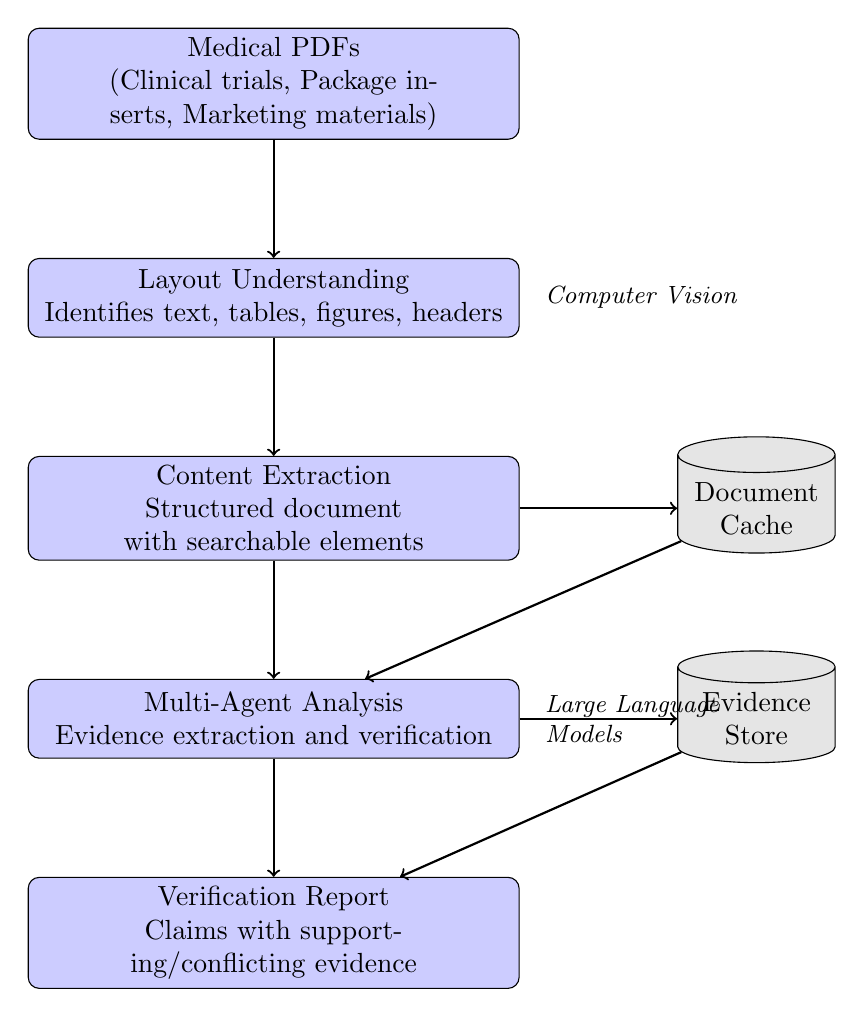
\begin{tikzpicture}[
    node distance=2cm,
    block/.style={rectangle, draw, fill=blue!20, text width=6cm, text centered, rounded corners, minimum height=1cm},
    decision/.style={diamond, draw, fill=orange!20, text width=4cm, text centered},
    data/.style={cylinder, draw, fill=gray!20, shape border rotate=90, aspect=0.25, minimum height=1cm, minimum width=2cm},
    arrow/.style={->,thick}
]

% Top level flow
\node[block, align=center] (pdf) {Medical PDFs\\(Clinical trials, Package inserts, Marketing materials)};
\node[block, below=1.5cm of pdf, align=center] (layout) {Layout Understanding\\Identifies text, tables, figures, headers};
\node[block, below=1.5cm of layout, align=center] (extract) {Content Extraction\\Structured document with searchable elements};
\node[block, below=1.5cm of extract, align=center] (agents) {Multi-Agent Analysis\\Evidence extraction and verification};
\node[block, below=1.5cm of agents, align=center] (report) {Verification Report\\Claims with supporting/conflicting evidence};

% Data stores
\node[data, right=2cm of extract, align=center] (cache) {Document\\Cache};
\node[data, right=2cm of agents, align=center] (evidence) {Evidence\\Store};

% Connections
\draw[arrow] (pdf) -- (layout);
\draw[arrow] (layout) -- (extract);
\draw[arrow] (extract) -- (agents);
\draw[arrow] (agents) -- (report);
\draw[arrow] (extract) -- (cache);
\draw[arrow] (cache) -- (agents);
\draw[arrow] (agents) -- (evidence);
\draw[arrow] (evidence) -- (report);

% Annotations
\node[text width=3cm, right=0.2cm of layout, font=\small\itshape] {Computer Vision};
\node[text width=3cm, right=0.2cm of agents, font=\small\itshape] {Large Language Models};

\end{tikzpicture}
\caption{High-level architecture of the Solstice system}
\end{figure}

\section{How It Works}

\subsection{Step 1: Understanding Document Structure}

Medical documents are complex—they mix narrative text with data tables, clinical figures, and regulatory disclaimers. Solstice first "sees" the document using computer vision to identify each element:

\begin{figure}[htbp]
\centering
\includegraphics[width=0.85\textwidth]{scientific_layout_example.png}
\caption{Layout detection on a clinical trial paper identifies distinct regions: title, abstract, body text, tables, and figures. Each element is extracted separately for targeted analysis.}
\end{figure}

This visual understanding is crucial because:
\begin{itemize}
\item Key efficacy data often appears in tables
\item Safety information may be in figure captions
\item Important disclaimers hide in footnotes
\item Marketing materials use visual hierarchy to emphasize claims
\end{itemize}

\subsection{Step 2: Intelligent Agent Orchestration}

Once the document structure is understood, specialized agents work together to verify claims:

\begin{figure}[htbp]
\centering
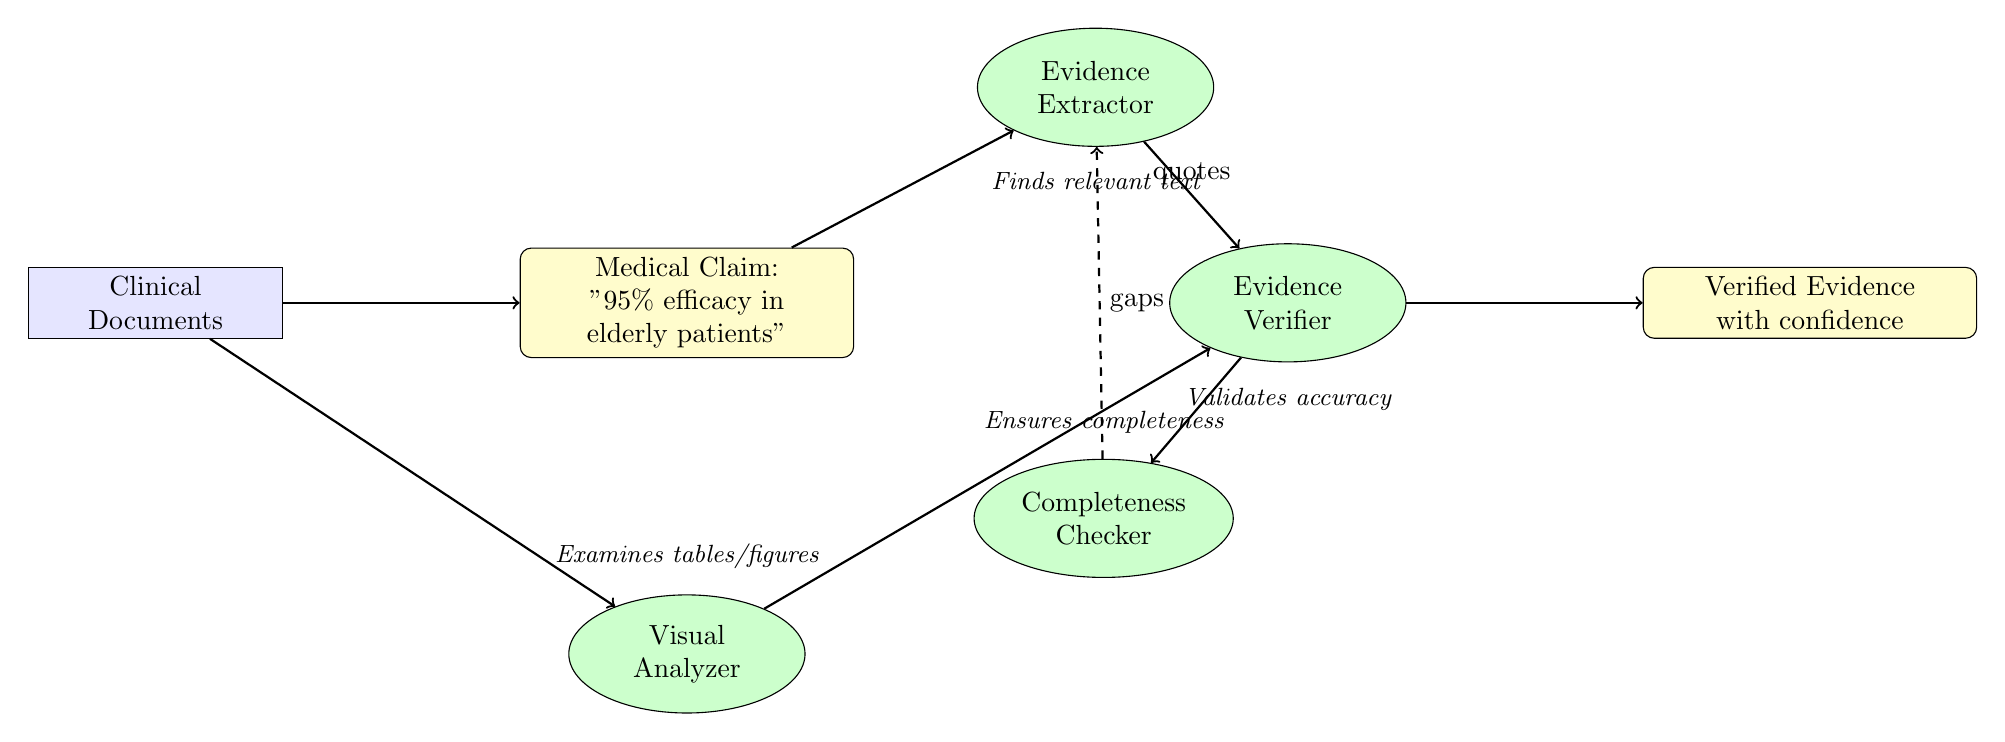
\begin{tikzpicture}[
    agent/.style={ellipse, draw, fill=green!20, minimum width=3cm, minimum height=1.5cm, text centered},
    claim/.style={rectangle, draw, fill=yellow!20, text width=4cm, text centered, rounded corners},
    doc/.style={rectangle, draw, fill=blue!10, text width=3cm, text centered},
    arrow/.style={->,thick},
    dasharrow/.style={->,thick,dashed}
]

% Center claim
\node[claim, align=center] (claim) {Medical Claim:\\"95\% efficacy in elderly patients"};

% Agents around the claim
\node[agent, above right=1.5cm and 2cm of claim, align=center] (extractor) {Evidence\\Extractor};
\node[agent, right=4cm of claim, align=center] (verifier) {Evidence\\Verifier};
\node[agent, below right=1.5cm and 2cm of claim, align=center] (checker) {Completeness\\Checker};
\node[agent, below=3cm of claim, align=center] (analyzer) {Visual\\Analyzer};

% Document source
\node[doc, left=3cm of claim, align=center] (doc) {Clinical\\Documents};

% Result
\node[claim, right=3cm of verifier, align=center] (result) {Verified Evidence\\with confidence};

% Connections
\draw[arrow] (doc) -- (claim);
\draw[arrow] (claim) -- (extractor);
\draw[arrow] (extractor) -- node[above] {quotes} (verifier);
\draw[arrow] (verifier) -- (result);
\draw[arrow] (verifier) -- (checker);
\draw[dasharrow] (checker) -- node[right] {gaps} (extractor);
\draw[arrow] (doc) -- (analyzer);
\draw[arrow] (analyzer) -- (verifier);

% Labels
\node[below=0.2cm of extractor, font=\small\itshape] {Finds relevant text};
\node[below=0.2cm of verifier, font=\small\itshape] {Validates accuracy};
\node[above=0.2cm of checker, font=\small\itshape] {Ensures completeness};
\node[above=0.2cm of analyzer, font=\small\itshape] {Examines tables/figures};

\end{tikzpicture}
\caption{Agents collaborate to thoroughly verify each claim, with feedback loops ensuring comprehensive coverage}
\end{figure}

Each agent has a specific role:
\begin{itemize}
\item \textbf{Evidence Extractor}: Searches documents for passages related to the claim
\item \textbf{Evidence Verifier}: Confirms quotes are accurate and truly support the claim
\item \textbf{Completeness Checker}: Identifies missing evidence and triggers additional searches
\item \textbf{Visual Analyzer}: Examines tables and figures for data supporting or contradicting claims
\end{itemize}

\subsection{Step 3: Comprehensive Reporting}

The system produces detailed reports showing:
\begin{itemize}
\item Exact quotes supporting each claim
\item Visual evidence from tables and figures
\item Conflicting information if found
\item Confidence assessment based on evidence strength
\item Missing evidence that couldn't be located
\end{itemize}

\section{Real-World Applications}

\subsection{Clinical Trial Verification}
When pharmaceutical companies publish trial results, Solstice can verify that marketing claims accurately reflect the scientific data. The system catches discrepancies like selective reporting or overgeneralization of results.

\subsection{Regulatory Compliance}
Medical device manufacturers must ensure their promotional materials align with FDA-approved indications. Solstice automatically cross-references marketing claims against regulatory documents.

\subsection{Marketing Material Review}

Marketing materials require special attention due to their persuasive nature:

\begin{figure}[htbp]
\centering
\includegraphics[width=0.85\textwidth]{marketing_layout_example.png}
\caption{Marketing materials use visual design to emphasize benefits. Solstice identifies promotional claims and verifies them against clinical evidence.}
\end{figure}

\section{Key Innovations}

\subsection{Multimodal Understanding}
Unlike text-only systems, Solstice analyzes tables, graphs, and figures—critical for medical evidence where key data often appears visually.

\subsection{Intelligent Orchestration}
Agents work together with feedback loops, ensuring thorough verification. If gaps are found, the system automatically searches for additional evidence.

\subsection{Traceable Verification}
Every claim links back to its source evidence, maintaining transparency and allowing human review of the automated findings.

\subsection{Scalable Architecture}
The system processes multiple claims in parallel while managing computational resources efficiently.

\section{Impact and Benefits}

\begin{itemize}
\item \textbf{Speed}: Reduces verification time from days to minutes
\item \textbf{Accuracy}: Systematic analysis eliminates human oversight errors
\item \textbf{Completeness}: Examines entire documents, not just keyword matches
\item \textbf{Transparency}: Provides traceable evidence for every verification
\item \textbf{Scalability}: Handles large document sets that would overwhelm human reviewers
\end{itemize}

\section{Future Directions}

Solstice continues to evolve with planned enhancements:
\begin{itemize}
\item Cross-document reasoning to synthesize evidence from multiple sources
\item Temporal analysis to track how claims change over time
\item Contradiction detection between related documents
\item Integration with regulatory databases for real-time compliance checking
\end{itemize}

\section{Conclusion}

Solstice represents a paradigm shift in medical document verification. By combining visual document understanding with intelligent agent orchestration, it transforms a manual, error-prone process into an automated, reliable system. This enables faster drug development, more accurate marketing, and ultimately, better-informed healthcare decisions.

\end{document}